\section{Knowledge Circuits Unveil Implicit Neural Knowledge Representations}

\paragraph{Knowledge Circuits Evaluation.}
We report the results of GPT2-Medium in Table~\ref{tab:completeness}, which indicates that with only less than 10\% of the original knowledge circuit’s subgraph, the model can maintain over 70\% of its original performance.
Additionally, we compute the random circuits by randomly deciding whether the edge should be removed and making sure the graph is connected. The random circuit is the same size as the circuit we discovered using our method. 
From the table, we can see that the random circuit failed to maintain the model’s performance, which further enhanced the robustness and efficacy of our methods.
One of the most fascinating observations is the \textbf{performance improvement seen on several test datasets}. 
For instance, the \emph{Landmark-country} relation metric increases from 0.16 to 0.36. 
This suggests that the discovered knowledge circuits may encapsulate the relevant knowledge, and the model's performance on these tasks could have been hindered by noise from other components.
We proceed to analyze the layer distribution of the original model $\mathcal{G}$ to understand the average percentage of nodes that are activated within the circuit for different knowledge domains. 
From Figure \ref{fig:layer_distribute}, we observe that attention and MLPs are more active in the lower layers of the network, where the language model processes the input and extracts general information.
To gain a more comprehensive view of the information processing, we compute the average $\operatorname{rank}_{o}$ change of the target token in the $D_{val}$ across the layers and report the results in Figure~\ref{fig:rank}. 
This analysis reveals the phenomenon of early decoding \cite{nostalgebraist_interpreting_nodate}, suggesting that by the middle to the latest layers, the target entity is already present in the residual stream, and the subsequent layers in the Transformer are designed to increase the probability of the current token (See discussion in the running example).
\begin{wrapfigure}{l}{0.42\columnwidth}
    \centering
    \vspace{-0.3cm}
    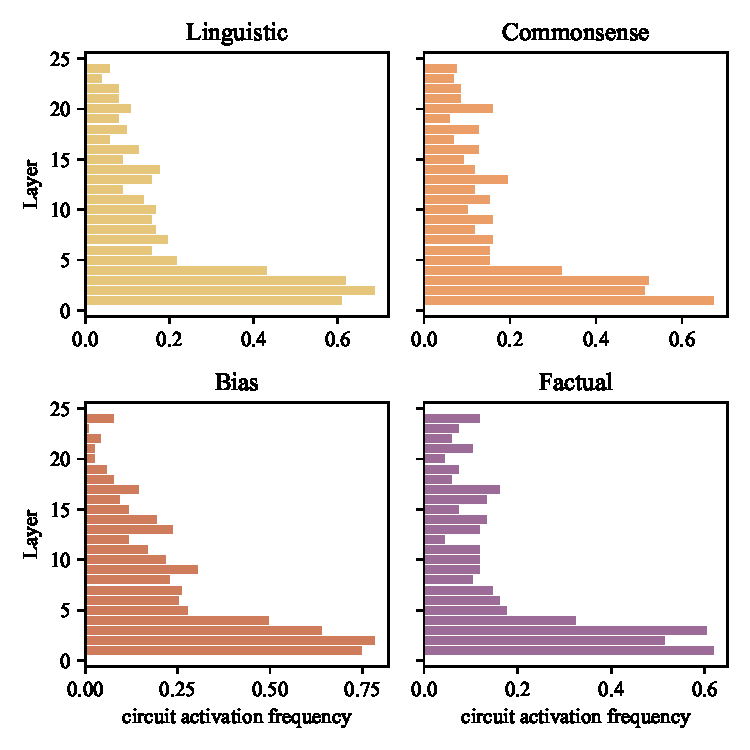
\includegraphics[width=0.99\linewidth]{Figure/layer_distribute.pdf}
    \caption{The activated circuit component distributions in Layers in GPT2-Medium.}
    \label{fig:layer_distribute}
    \vspace{-0.5cm}
\end{wrapfigure}
\paragraph{Special Components in Knowledge Circuits.}
From the discovered knowledge circuits, we can find several important attention heads that demonstrate specific behavior, including the \textbf{mover head}~\cite{lv2024interpreting}, \textbf{relation head}~\cite{chughtai2024summing,ferrando2024primer} and \textbf{mixture head}~\cite{chughtai2024summing,ferrando2024primer} (more definitions in Appendix~\ref{app:definition}).
Mover Head~\cite{lv2024interpreting,merullo2023circuit} focuses on the last token of the context and attends to the subject token, functioning as a mover to transfer information, while Relation Head~\cite{chughtai2024summing} attends to the relation token in the context and produces some relation-related tokens that would guide the behavior of the following components.
We think that these components would be accumulated by the MLP in the model, and the behavior of these special heads will be discussed in the running example part.
We list some of these special components in Table \ref{tab:component} in Appendix. 
The different attention heads are responsible for expressing specific types of knowledge and may be activated by different facts.
In our experiments with GPT-2 Medium and GPT-2 Large, we find that knowledge is distributed across several layers' attention heads and MLP matrices, suggesting that the target knowledge appears to have been accumulated throughout the GPT-2 model.
Conversely, in TinyLLAMA, the special components are more concentrated.
As depicted in Figure \ref{fig:rank}, the rank of the target entity in TinyLLAMA experiences a sharp decline around several layers, whereas in the GPT2 model, the decline is more gradual. 
We hypothesize that this discrepancy may be attributed to the model's knowledge capacity \cite{knowledge_capacity} and warrants further investigation.
\paragraph{A Running Example of Knowledge Circuit.}
\label{sec:case_results}

We present a case and analyze the specific behaviors of components within the identified knowledge circuits.
In particular, we find some special attention heads in the model such as the mover head and the relation head. 
We demonstrate the function of these heads in Figure~\ref{fig:head_function} by ablating them from the circuit.
Taking the factual knowledge \nl{The official language of France is French} as an example, we visualize the knowledge circuit in Figure \ref{fig:circuit}.
To express the information flow within the model more effectively, we have plotted the rank and probability of the target entity $o$ at each layer when it is mapped into the embedding space, in Figure~\ref{fig:case_layer}. 
From this figure, we can see that after MLP 17, the target knowledge emerges as the top token in the residual stream, and after that layer, it undergoes an increased probability.
The edges connected to MLP17 are (L14H13 $\rightarrow$ MLP17), (L14H7 $\rightarrow$ MLP17), and (L15H0 $\rightarrow$ MLP17) .
Here, the L14H13 is a relation head that focuses on the relation token in the context.
The output of this head is relation-related tokens such as \nl{language} and \nl{Language}.
The attention head L14H7 is a mover head that moves the information from the subject position \nl{France} to the last token. 
Previous work~\cite{lv2024interpreting,merullo2024language} has introduced this mover head as an \emph{argument parser}, which moves \nl{France} to the last token, and the subsequent MLP conducts a function application to map \nl{France} to \nl{French}. 
An intriguing observation is that we can find the output of this head already contains the target answer entity, which significantly contributes to the final output (L14H7 $\rightarrow$ Output).
Also, we see the probability of the subject token in Figure~\ref{fig:case_layer} at the last token is nearly zero across these layers.
Hence, instead of the \emph{argument parser} function, we consider this mover head as an \emph{extract head} proposed by \citet{geva-etal-2023-dissecting}, which aims to extract the related-information from the subject token's position.
In the subsequent knowledge editing experiments, we can observe changes in the behavior of these types of heads. 
\begin{wrapfigure}{r}{0.45\columnwidth}
    \centering
    \vspace{-0.3cm}
    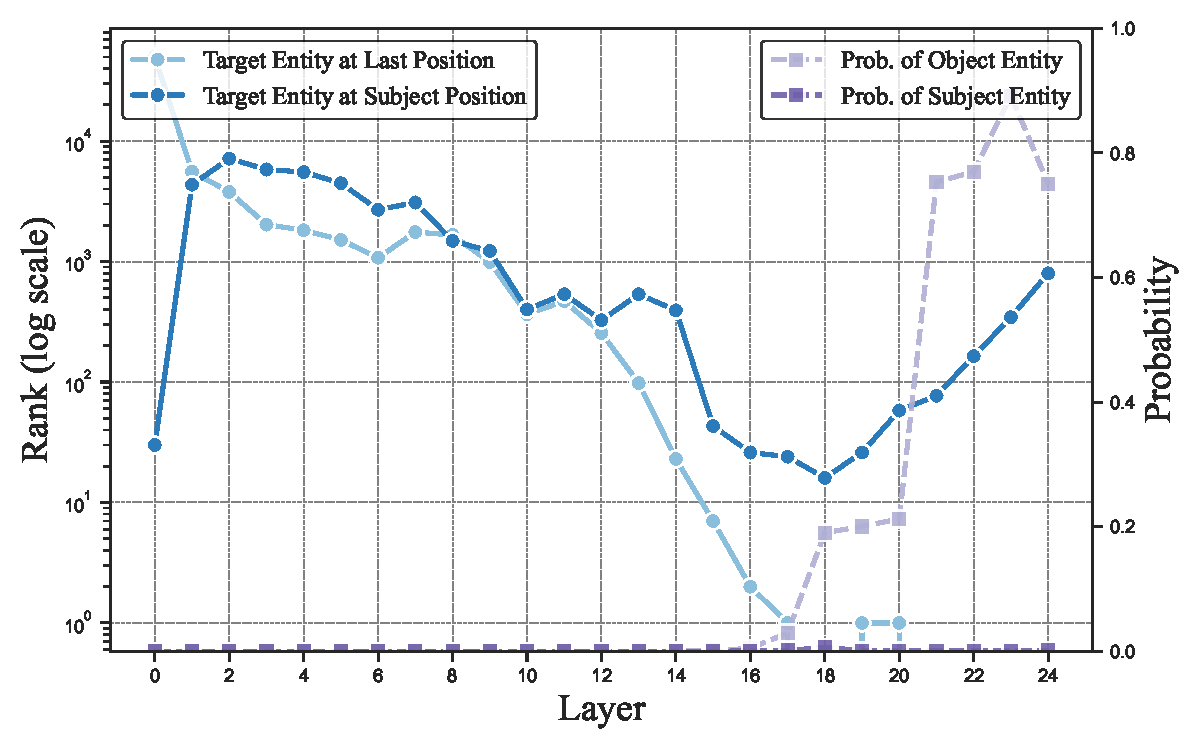
\includegraphics[width=0.99\linewidth]{Figure/newoutput.pdf}
    \caption{The rank and probability of the target entity $o$ at both the last subject token and the last token position when unembedding the intermediate layer's output for the fact \nl{The official language of France is French}. }
    \label{fig:case_layer}
    \vspace{-0.1cm}
\end{wrapfigure}
Additionally, instead of extraction in the later layers proposed by \citet{geva-etal-2023-dissecting}, we notice a gradual decrease in rank across all early-to-middle layers.
The MLP17 combines information from previous tokens and integrates this information to prioritize the target token at the top rank.

Interestingly, upon tracing the information flow to L14H7, we discovered that it is predominantly activated by L7H14, a relation head, and its output features several language tokens, such as \nl{Arabic}.
We hypothesize that L7H14 may function as a signaling mechanism to activate the associated mover head, but this hypothesis necessitates further investigation to be confirmed. 
After MLP17, several attention heads, such as L18H14 (a relation head) and L20H6 (a mover head), collaborated to further enhance the final prediction of the target entity.
% Here, the L14H13 is a relation head that focuses on the relation token in the context. Its output contains relation-related tokens such as "language" or "Language." The attention head L14H7 is a mover head that transfers the information of the subject "France" to the last token. An interesting aspect is that the output of this head already contains the target entity, which significantly contributes to the final output (L14H7 $\rightarrow$ Output). The MLP17 combines the previous tokens and consolidates the information, pushing the target token to the top rank.
% Tracing back the information for L14H7, we can find that its primary input comes from the L7H14, which is also a mover head. There are other similar attention heads, such as L18H14 and L20H6, that work together to enhance the final prediction of the target entity.
% This detailed analysis of a specific circuit illustrates the intricate information processing and knowledge representation within the language model. It provides insights into the specific components and their interactions that lead to the correct prediction of the target entity in this context.